% Title and author information 
\title{EXPERIMENTAL CHARACTERIZATION OF POLARIZED LASERS}
\author{
    Eduardo Barroso \address{1} \\[0.3em]
    {\scriptsize
        \address{1} Department of Physics Engineering; Monterrey Institute of Technology, Monterrey, N.L 64849.\\
    }
}
\date{\today}


\setabstract{
    The transversal nature of electromagnetic waves gives rise to a characteristic of light called polarization. 
    It is by studying polarization that we can construct optical systems that enable physicists to exploit the wave nature of light. 
    The following work aims to expose a complete process of characterizing the polarization state of a LASER beam. 
    First, a brief framework is constructed on Polarization theory. 
    Then, characterization techniques are presented in a sequential way; building from linear to circular polarization. 
}

\maketitle
    
\section{Introduction}
\label{sec:INTRO}
Most sources of light can be characterized as non polarized, de-coherent and transversal electromagnetic waves. This means that light rays - for instance from the sun - are composed of transversal electromagnetic oscillations with random spatial orientations and temporal decoherence. However, in its simplest and purest form, light has a preferred spatial orientation as shown in figure \ref{fig:PolvNPol}. This state of light is referred to as polarized light.\\

This work aims to explain a complete process of characterizing the polarization of a LASER beam. This is with the objective of reinforcing the basic principles behind polarization through hands-on experimentation. The team creates a empirical argument of how polarized light behaves when subjected to different optical elements. 

\section{Materials}

\begin{enumerate}
    \item LASER HeNe (633nm, 15mW)
    \item 2 Linear Polarizators.
    \item 2 Retarder of quarter wavelength.
    \item 1 Retarder of half wavelength.
    \item Power / Intensity Measurement device. 
    \item Fixed Optic Mounts.
    \item 2 Mirrors.
    \item 1 Collimator.
    \item 1 Pupil.
    \item Security Glases.
\end{enumerate}

\section{Theoretical Framework}
\label{sec:TEO_FRAMEWORK}
%%%%%%%%%%%%%%%%%%%%%%%%%%%%%
\subsection{ELECTROMAGNETIC WAVES}
An electromagnetic wave as shown in figure \ref{fig:PolvNPol} can be characterized by its amplitude ($E_o$), frequency ($w$), phase ($\phi$), direction of the wave ($\Vec{k}$) but also the direction of displacement ($\Vec{P}$). Note that these last vectors are not the same. The former ($\Vec{k}$) refers to the direction in which the light ray propagates and the latter refers to the direction of oscillation. 

\textbf{Def. Polarization}: The direction of the displacement vector is called the \textit{direction of polarization}. Furthermore the plane on which this vector lives and oscillates is the plane of polarization \cite{guenther2015modern}. 
\begin{figure}[H]
    \centering
    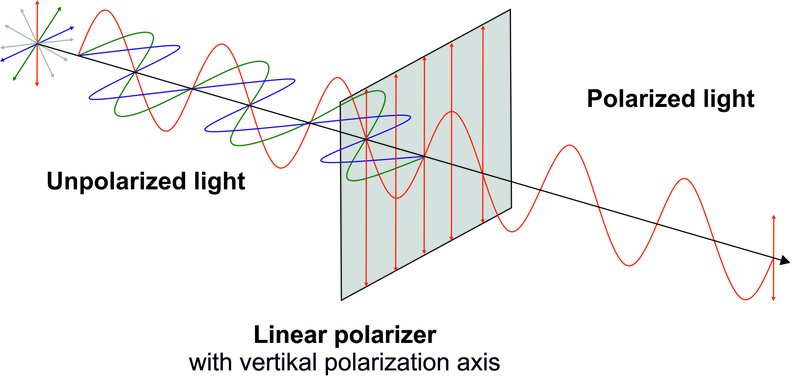
\includegraphics[scale=0.80]{Figures/Polarization_NonPolarization.jpg}
    \caption{Polarized vs Non Polarized light}
    \label{fig:PolvNPol}
\end{figure}

\textbf{On the nature of Circular Polarization}\\
A very interesting state of polarization is circular polarization. When we introduce a phase difference equal to $\pi/2$ between the two perpendicular and constituent \footnote{A state of polarization can be mathematically modeled as a vector containing a direction $\hat{x}$ and $\hat{y}$} components of light, the resulting vector of polarization ($\Vec{P}$) propagates in time and space in one of two ways: (i) circular orbits if the components have the same amplitudes or (ii) elliptical orbits if there exists a difference between the components amplitudes. Figure \ref{fig:CircularPol} illustrates this state.

\begin{figure}[H]
    \centering
    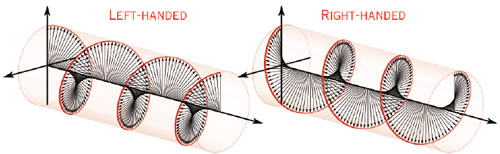
\includegraphics[scale=0.40]{Figures/Circular_Polarization.jpg}
    \caption{Circular Polarization Illustration (N.A)}
    \label{fig:CircularPol}
\end{figure}

One of the biggest misconceptions about this state of polarization is that at any given instant, the polarization state is a circle. Truth is that circular polarization is an emergent illusion that is due to the perpendicular components oscillating out of phase by exactly $pi/2$. This quantity can also be related to the wavelength of the beam. For this case this relation is $\lambda/4$.

%%%%%%%%%%%%%%%%%%%%%%%%%%%%%
\subsection{OPTICAL ELEMENTS}
The main elements for characterizing the polarization of a beam are presented in this section. \\

\textbf{Def. Polarizer:} A polarizer is an optical element that only allows one direction of polarization to be transmitted. For instance, a diagonal polarization incident on a vertical polarization will lose its horizontal component and the transmitted wave will be vertical. \\


\textbf{Def. Retarder:} This type of plate has two different refraction indices on its main perpendicular axis. The axis with a smaller refractive index ($n_f$) will be the fast axis, the other axis with $n_s$ will be the slow axis. Both refractive indices relate to the thickness ($d$) of the element by the relation
\begin{equation}
    d = \frac{\lambda}{4(n_s-n_f)}.
    \label{eq:retard}
\end{equation}
Equation \ref{eq:retard} states a retarder is dependent on the wavelength ($\lambda$) of the beam that is incident. The other key takeaway is that these elements introduce a difference in phase on the components of the light by allowing one component to move fast and the other slow. We will refer to this difference in phase as $\psi$ when we present the experimental results.  


%%%%%%%%%%%%%%%%%%%%%%%%%%%%%
\subsection{MALUS LAW}
Mauls Law is a straight forward mathematical derivation of the power or intensity of a polarized light ray as the polarizer rotates along the optical axis a given angle $\theta$. The relation

\begin{equation*}
    I_{tot} = I_{max}*cos(\theta),
\end{equation*}
is a power full tool to determine a certain state of polarization by measuring the intensity experimentally with previous knowledge of the maximum value $I_{max}$.

%%%%%%%%%%%%%%%%%%%%%%%%%%%%%
\subsection{STOKES PARAMETERS}
The stokes parameters yield information about the polarization state of a particular beam of light. Furthermore, they can be measured in experiments an hence serve as a practical tool that helps when characterizing optical systems. The parameters are the following: 
\\
\begin{enumerate}
    \item $S_0 = |E_x|^2 + |E_y|^2 $\\
    Total power density
    \item $S_1= |E_x|^2 - |E_y|^2 $ 
    Difference between power density transmitted by 2 perpendicular directions of polarization; horizontal and vertical.
    \item $S_2= |E_d|^2 - |E_ad|^2$ 
    Difference between power density transmitted by 2 perpendicular directions of polarization; diagonal and anti-diagonal.
    \item $S_3= |E_R|^2 - |E_L|^2$ 
    Difference between power density transmitted by 2 perpendicular directions of polarization; circular right and left. 
\end{enumerate}

A more elegant way of visualizing such parameters is with a Poincare Sphere (Figure \ref{fig:Poincare}). In this phase space, each axes represent a possible polarized state. A vector within this sphere is a possible polarization state for light. 
\begin{figure}[H]
    \centering
    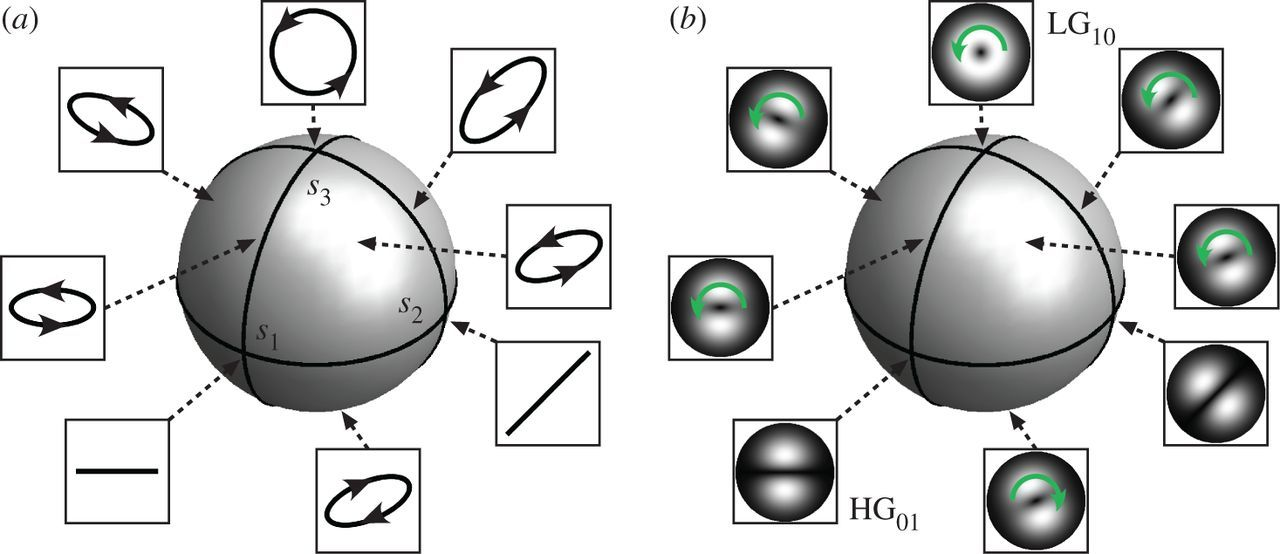
\includegraphics[scale=0.70]{Figures/Poincare.jpg}
    \caption{Poincare Sphere \cite{figpoincare}}
    \label{fig:Poincare}
\end{figure}



\section{Results}
\label{sec:RESULTS}

\subsection{CHARACTERIZATION OF LINEAR POLARIZATION}
First, we align the lazer by adjusting the two mirrors in our optical arrangement. This is important in order to ensure a fixed and straight optical path throughout our optical elements.\\

\begin{figure}[H]
    \centering
    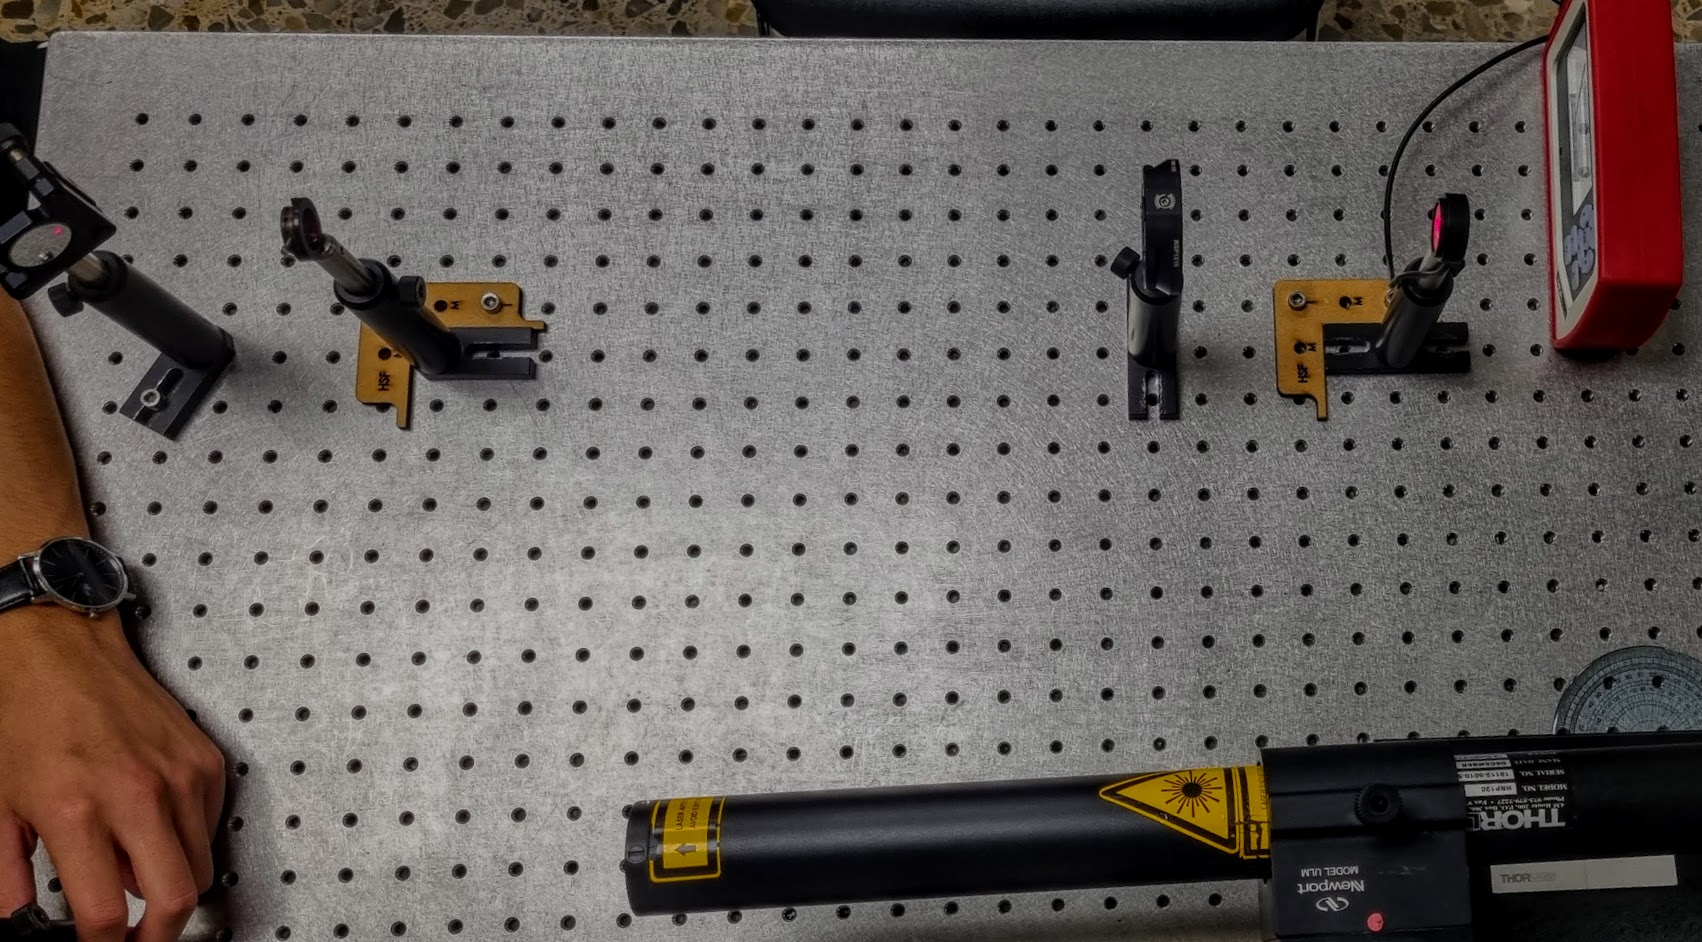
\includegraphics[scale=0.14]{Figures/Polarization_1setup.jpg}
    \caption{LASER (Bottom Right), aligned mirrors (left side), polarizer (center right) and intensity measurement device (far right).}
    \label{fig:Setup1}
\end{figure}

Once the LASER is aligned, we setup the polarizer and the intensity measurement device. We rotate the polarizer until we obtain a maximum and a minimum value. The values are presented in table \ref{Tab:LPs}\\ 

\begin{table}[H]
\begin{center}
\begin{tabular}{|l|l|l|}
        & Intensity  & Angle        \\
Maximum & 10.63 $mW$ & 357 $degree$ \\
Minimum & 0.02 $mW$  & 87 $degree$ 
\end{tabular}
\caption{Measurements of Maxima of the LASER}
\label{Tab:LPs}
\end{center}
\end{table}

Because these extrema angles are perpendicular to each other it is possible to conclude that the LASER-beam is linearly polarized. However because the polarizer does not indicate its orientation of polarization, we are not able to determine the polarization of the beam.  \\

To determine the orientation of the polarizer it is necessary to find a source of polarized light with a known linear polarization \footnote{An example of such source can be light reflected from a surface at Brewster angle or a digital screen. }. For such source, the team used a digital screen to determine that at the 100 degree mark, the polarizer blocks the vertical polarization of the screen (Figure \ref{fig:FOR}). \\

\begin{figure} [H]
    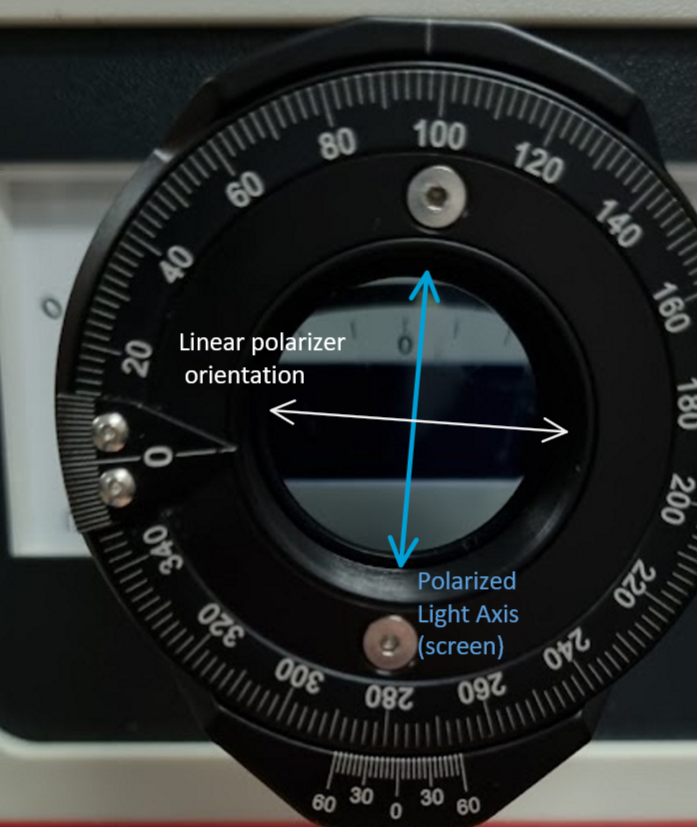
\includegraphics[width=.20 \textwidth]{Figures/Polarization_FrameoRef_Real.png}\hfill
    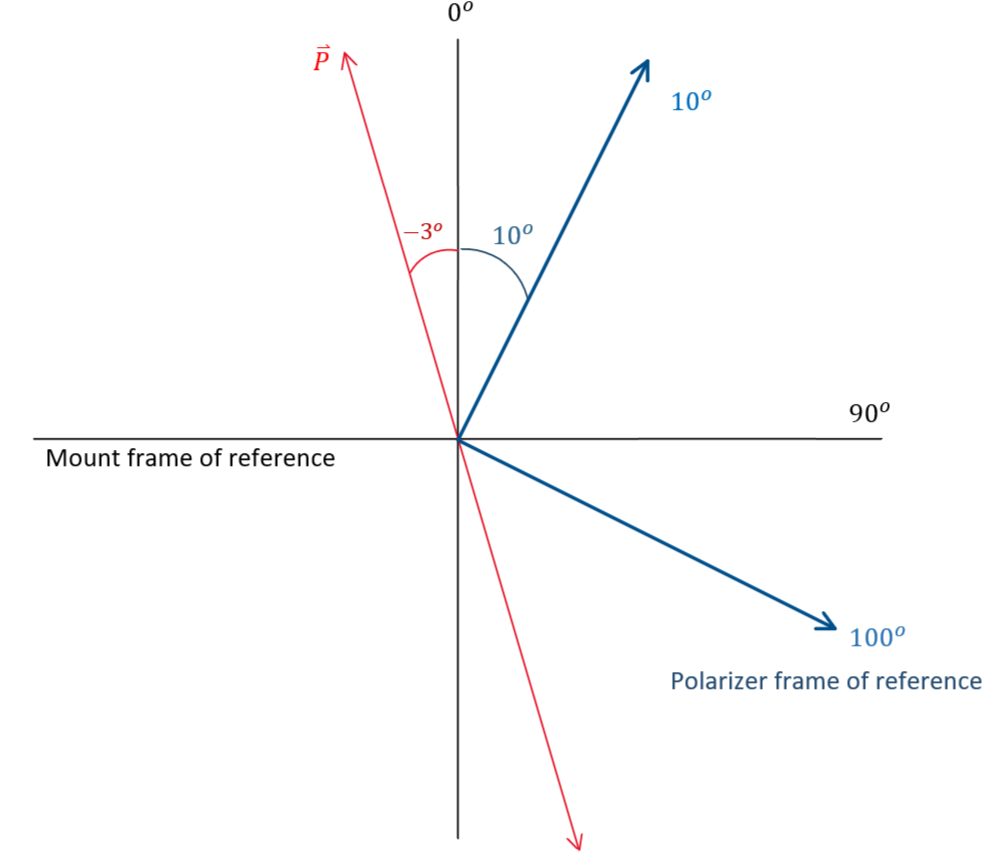
\includegraphics[width=.26\textwidth]{Figures/Polarization_FrameoRef.png}\hfill

    \caption{Polarization Diagrams used to determine polarization}\label{fig:FOR}
\end{figure}

This leads us to conclude that the LASER beam in our setup has anti-diagonal polarization ($\Vec{P}$) with a $-13^o$ degree shift with respect to the polarizer frame of reference. A diagram illustrating the previous results is presented in figure \ref{fig:FOR}. \\

\subsection{EMPIRICAL PROOF OF MALUS LAW}
Rene Descartes once said "The conquest of nature is to be achieved through number and measure". In section \ref{sec:TEO_FRAMEWORK}, we exposed that Mauls Law is a simple mathematical derivation that uses basic geometrical considerations about  light and leads to a relation between the polarizer, the polarized beam and the intensity or power \footnote{For practical purposes, we do not differentiate between intensity and power.}. In this section, the team aims to test experimentally that this law holds for our arrangement. \\

To test this law, the team uses the setup exposed in figure \ref{fig:Setup1}.We start to vary the angle of the polarizer and take discrete measurements of intensity (Figure \ref{fig:Setup2}). After the data is collected, a few considerations are taken into account to calibrate and define the angle $0^o$. The results obtained are presented in the figure \ref{fig:Malus}. \\

\begin{figure}[H]
    \centering
    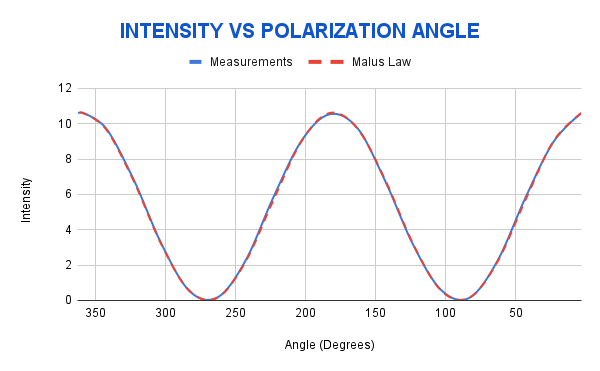
\includegraphics[scale=0.33]{Figures/INTENSITY VS POLARIZATION ANGLE .png}
    \caption{Test of Malus Law}
    \label{fig:Malus}
\end{figure}

The results leads us to state that Mauls law holds in our experiment. After a care-full study of the difference in values, the team obtained a relative error of $1.04\%$. The fact that we proved empirically that measurements match the theory lets us use Malus law as a tool in future characterizations with a high certainty.

\begin{figure} [H]
    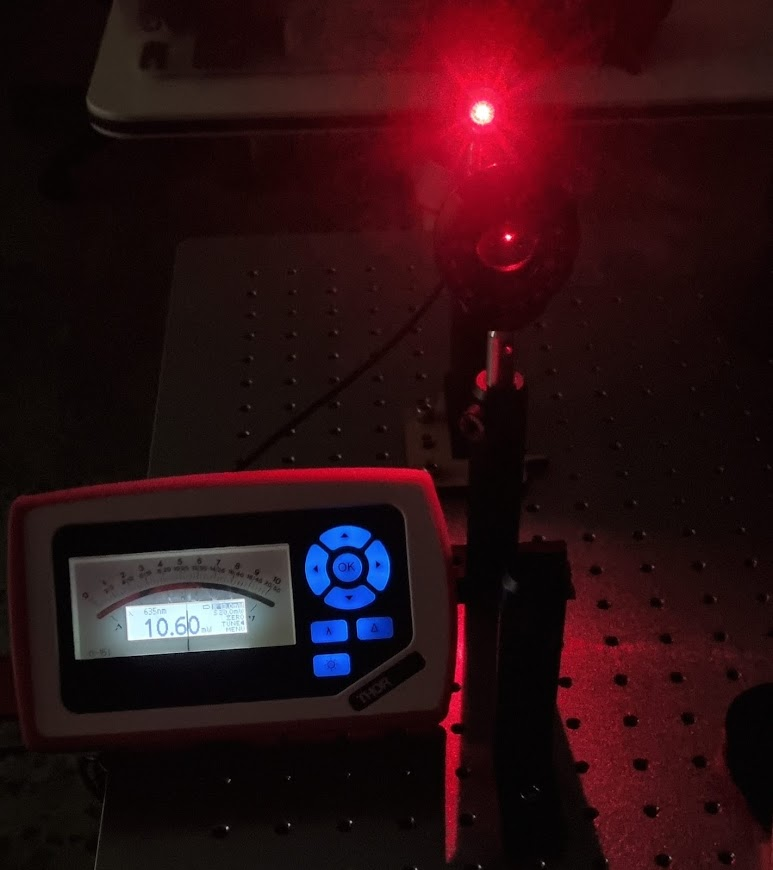
\includegraphics[width=.23\textwidth]{Figures/Polarization_Setup2.1.jpg}\hfill
    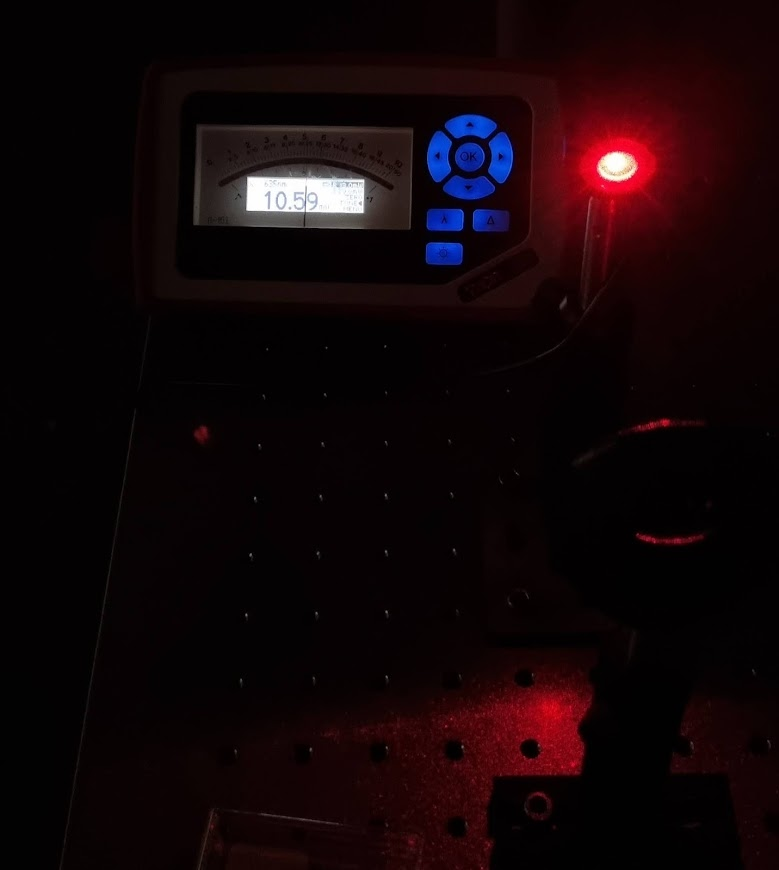
\includegraphics[width=.23\textwidth]{Figures/Polarization_Setup2.2.jpg}\hfill
    \caption{Polarization setup to test Malus Law}
    \label{fig:Setup2}
\end{figure}

\subsection{INDUCE A CIRCULAR POLARIZATION}
The arrangement presented in figure \ref{fig:CircularPolS1} is made in order to generate and characterize circular polarization.
\begin{figure}[H]
    \centering
    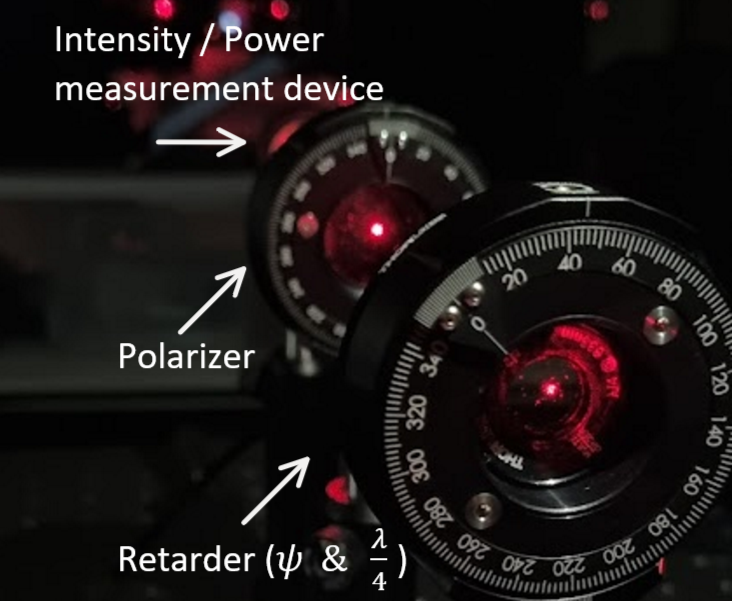
\includegraphics[scale=0.30]{Figures/Polarization_Setup3.png}
    \caption{Circular polarization setup}
    \label{fig:CircularPolS1}
\end{figure}
First, the team varied the angle on the retarder until we obtained a value of intensity of $10.57 mW$. At this configuration we state that the linear polarized LASER orientation is parallel to the orientation of the fast (or slow) axis of the retarder plate. To verify such statement the team proceeded to vary $90$ degrees the angle of the retarder and we obtained another maxima of $10.40 mW$. This means that now the LASER polarization is perfectly parallel to the other axis of the retarder. Then, we proceeded to vary the retarder angle $-45$ degrees to induce circular polarization. We can verify that we obtained this state by varying the polarizer angle. Since its circular polarization, we expect to have minimum variations in intensity as we vary the polarizer orientation since the polarized state is rotating in time in all orientations. To the teams satisfaction, the results of varied between $5.11 mW$ and $5.53 mW$. These values correspond to half of the total intensity because at any given angle, the polarizer blocks half of the energy that the circular polarization has. \\

\subsection{INDUCE A PERPENDICULAR POLARIZATION}
Just as we have retarders of $\psi = pi/2$, there are retarders that introduce a phase difference of $pi$ or $\lambda/2$ to polarized states. The effect of such elements are that they rotate the state of polarization by $90$ degrees. \\

To induce such polarization, the team took the setup presented in \ref{fig:Setup2} and change the $\lambda/4$  retarder to a $\lambda/2$ retarder. When such element was introduced the intensity measurement was $0.00 mW$ this is because the polarizer in front of the retarder was oriented to allow vertical polarization and the retarder induced a horizontal polarization on the incident vertical polarization.  


\subsection{CHARACTERIZATION OF CIRCULAR POLARIZATION WITH STOKES PARAMETERS}
From a practical standpoint, the Stokes parameters narrow down to 4 simple questions: (i) How much intensity or power a given light source has, (ii) How much is it polarized in the horizontal-vertical direction, (iii) How much is it polarized in the diagonal-anti diagonal direction and (vi) How much is it polarized in the circular L-R direction? For this reason, it is of great interest for physicists that try to characterize light in experimental setups to determine. \\

To determine these parameters for circular popularization states, the team built the following optical system presented in figure \ref{fig:Setup2} once again inserting the  $\lambda/4$ retarder. Later, we varied the linear polarizer to obtain the following measurements for each polarization state (Table \ref{Tab:Stokes}). \\

\begin{table}[H]
\begin{center}
\begin{tabular}{|l|l|l|l|}
      & $E_1$ & $E_2$ & Value \\
$S_0$ & 5.27  & 5.28  & 10.55  \\
$S_1$ & 5.27  & 5.28  & -0.01   \\
$S_2$ & 5.46  & 5.44  & 0.02     \\
$S_3$ & 10.49 & 0.01  & 10.48       
\end{tabular}
\caption{Measurements of Stokes Parameters}
\label{Tab:Stokes}
\end{center}
\end{table}

Finally, with the same setup we introduced a $\lambda/2$ retarder. After making the same measurements of the stokes parameters we obtained similar results but with the $S_3$ with a negative value. This result tells us that the circular polarization was inverted due to the  $\lambda/2$ retarder. The results are presented in table \ref{Tab:Stokes2}.
\begin{table}[H]
\begin{center}
\begin{tabular}{|l|l|l|l|}
      & $E_1$ & $E_2$ & Value \\
$S_3$ & 0 & 10.39  & -10.39       
\end{tabular}
\caption{Measurements of Stokes Parameters with $\lambda/2$ retarder}
\label{Tab:Stokes2}
\end{center}
\end{table}
The mathematical description of this polarized states represent vectors. The optical elements represent matrices - Called Jones matrices. With a simple knowdlege of linear algebra its easy to understend the numerical description of the system presented in figure \ref{fig:Proof}. 
\begin{figure}[H]
    \centering
    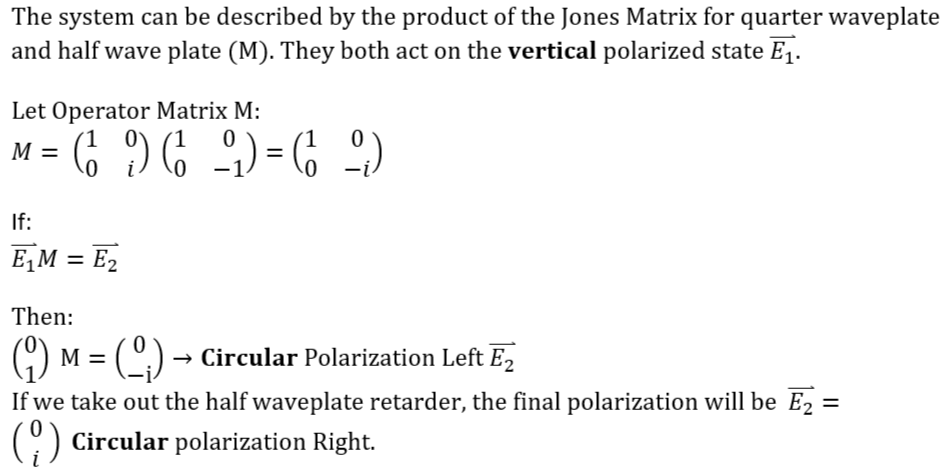
\includegraphics[scale=0.42]{Figures/Proof.png}
    \caption{From vertical to circular polarization}
    \label{fig:Proof}
\end{figure}

\section{Conclusion}
Light is a natural phenomena that can be manifested in many different ways. Depending on the state of the light, emergent phenomena like interference and coherence can occur. Furthermore, the practical applications of this phenomena yield excellent promising technologies that can be sized down down to the scale of nanometers. Therefore, it is very important to have characterization tools when dealing with optical systems given the many states of polarization a beam can have.\\


Thought this work, we exposed the principal characterization techniques when dealing with polarized light. Finally, the team concludes that  success-full measurements where obtained. The empirical characterizations exposed reinforced the contents discussed on the optical experimentation course. 

% References
%\onecolumn
\printbibliographysection{Polarization Practice References}
%\twocolumn